The code for all the experiments described in this section are available at the following link : \url{https://github.com/MaxenceGiraud/ucb-nonstationary}.

We performed three different experiments using the five algorithms described in this paper. The first one is the original UCB-1 used as a baseline for all the experiments. The second one is Disounted UCB, and the last three are the Sliding Window UCB described by Garivier et al. \cite{garivier2008upperconfidence} and the two variants we talked about in the last section.\\
The parameters of the policies were tuned as Garivier et al. did. This means with for all algorithms $\xi = 0.5$, $\gamma = 1 - \frac{1}{4\sqrt{T}}$ and $\tau = 4 \sqrt{K \log(T)}$. As an example for $T=1000$ and $K=3$, $\tau = 18$ and $\gamma = 0.992$.\\

The first experiment consists of a simple stationary problem with three Gaussian with means respectively 0.2, 0.3 and 0.4. The results are displayed on figure \ref{fig:statio}. As we expected the original UCB performed much better than all the other algorithms. One justification of the poor performance in the case of the main policy of interest Sliding Window UCB, can be that it has to draw each arm at least $T/\tau$ times and so even if one arm is consistently better than the others, it will draw it consequent number of times.\\

\begin{figure}[ht]
    \centering
    \begin{subfigure}{.6\textwidth}
      \centering
      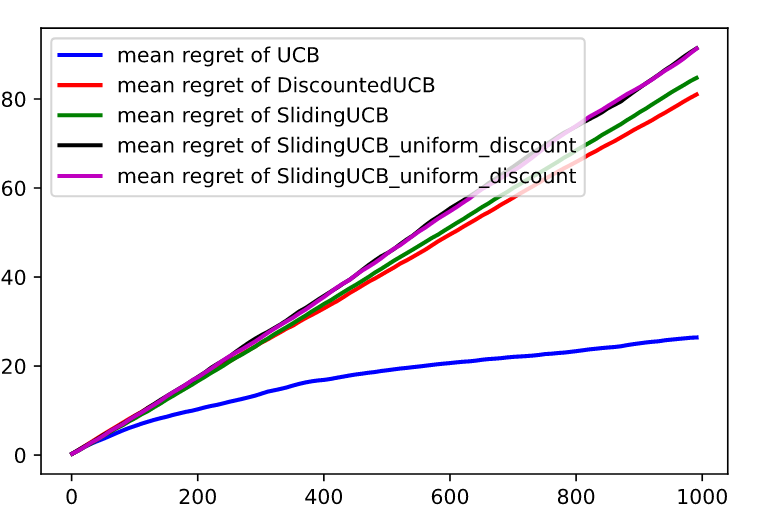
\includegraphics[width=.8\linewidth]{img/statio.png}
      \caption{Stationary Bandit}
      \label{fig:statio}
    \end{subfigure}%
    \begin{subfigure}{.6\textwidth}
      \centering
      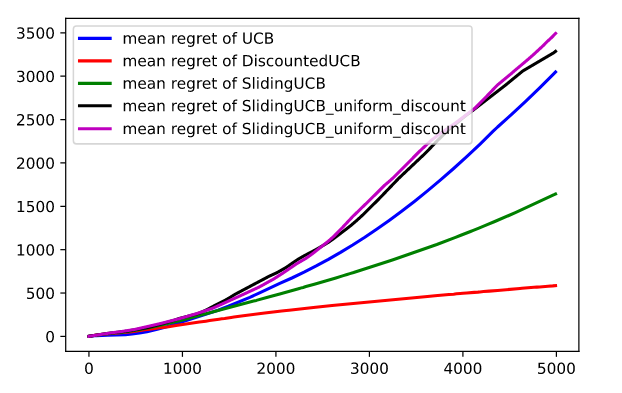
\includegraphics[width=.8\linewidth]{img/continuous.png}
      \caption{Continuously changing MAB}
      \label{fig:conti}
    \end{subfigure}
    \begin{subfigure}{.6\textwidth}
        \centering
        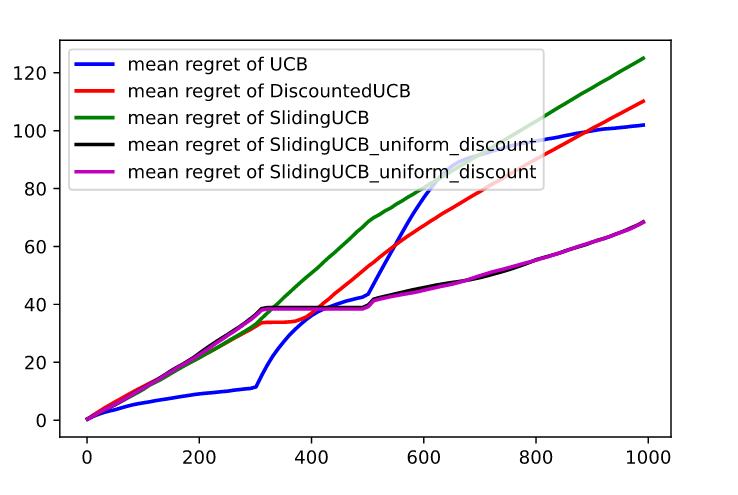
\includegraphics[width=.8\linewidth]{img/abrupt.png}
        \caption{Abrubtly changing MAB}
        \label{fig:abrupt}
      \end{subfigure}
\end{figure}


The second experiment consists of a continuously changing environment. We kept two arms stationary which are Gaussians of means 0.2 and 0.7 while the third is a Gaussian with a mean dependant of the time t: $0.4 + \frac{t}{T}$. The results are reported in figure \ref{fig:conti}.\\
Again as expected, the best performing policy is the Discounted UCB which is design for this kind of environment. We also found as in the studied paper that the Sliding UCB is still performing quite well on this problem, while our two variants fail and do worse than a standard UCB.\\

The last experiment is the main study of the paper, is the abruptly changing environment. It is modeled as follows: two arms do not change over time and are represented by Bernouilli with parameters respectively 0.5 and 0.4. And a third arm that for $T < 300 $ and $T > 500$ it is modeled as a Bernouilli with probability equals to 0.1 while in the interval it is 0.9. The results of this third experiment are reported in figure \ref{fig:abrupt}.\\
Here the best performing algorithm is actually our first variant (the Sliding UCB with Uniform Discount) while Sliding UCB is the worse performing one. We cannot firmly conclude over these results as firstly they contradict the ones from the paper, and secondly due to a lack of machines that could perform long tasks ($T>10000$) a sufficient number of times for the experiment to be statistically conclusive.